% Options for packages loaded elsewhere
% Options for packages loaded elsewhere
\PassOptionsToPackage{unicode}{hyperref}
\PassOptionsToPackage{hyphens}{url}
%
\documentclass[
  ignorenonframetext,
]{beamer}
\newif\ifbibliography
\usepackage{pgfpages}
\setbeamertemplate{caption}[numbered]
\setbeamertemplate{caption label separator}{: }
\setbeamercolor{caption name}{fg=normal text.fg}
\beamertemplatenavigationsymbolsempty
% remove section numbering
\setbeamertemplate{part page}{
  \centering
  \begin{beamercolorbox}[sep=16pt,center]{part title}
    \usebeamerfont{part title}\insertpart\par
  \end{beamercolorbox}
}
\setbeamertemplate{section page}{
  \centering
  \begin{beamercolorbox}[sep=12pt,center]{section title}
    \usebeamerfont{section title}\insertsection\par
  \end{beamercolorbox}
}
\setbeamertemplate{subsection page}{
  \centering
  \begin{beamercolorbox}[sep=8pt,center]{subsection title}
    \usebeamerfont{subsection title}\insertsubsection\par
  \end{beamercolorbox}
}
% Prevent slide breaks in the middle of a paragraph
\widowpenalties 1 10000
\raggedbottom
\AtBeginPart{
  \frame{\partpage}
}
\AtBeginSection{
  \ifbibliography
  \else
    \frame{\sectionpage}
  \fi
}
\AtBeginSubsection{
  \frame{\subsectionpage}
}
\usepackage{iftex}
\ifPDFTeX
  \usepackage[T1]{fontenc}
  \usepackage[utf8]{inputenc}
  \usepackage{textcomp} % provide euro and other symbols
\else % if luatex or xetex
  \usepackage{unicode-math} % this also loads fontspec
  \defaultfontfeatures{Scale=MatchLowercase}
  \defaultfontfeatures[\rmfamily]{Ligatures=TeX,Scale=1}
\fi
\usepackage{lmodern}

\usetheme[]{CambridgeUS}
\usefonttheme[]{professionalfonts}
\ifPDFTeX\else
  % xetex/luatex font selection
\fi
% Use upquote if available, for straight quotes in verbatim environments
\IfFileExists{upquote.sty}{\usepackage{upquote}}{}
\IfFileExists{microtype.sty}{% use microtype if available
  \usepackage[]{microtype}
  \UseMicrotypeSet[protrusion]{basicmath} % disable protrusion for tt fonts
}{}
\makeatletter
\@ifundefined{KOMAClassName}{% if non-KOMA class
  \IfFileExists{parskip.sty}{%
    \usepackage{parskip}
  }{% else
    \setlength{\parindent}{0pt}
    \setlength{\parskip}{6pt plus 2pt minus 1pt}}
}{% if KOMA class
  \KOMAoptions{parskip=half}}
\makeatother

\usepackage{color}
\usepackage{fancyvrb}
\newcommand{\VerbBar}{|}
\newcommand{\VERB}{\Verb[commandchars=\\\{\}]}
\DefineVerbatimEnvironment{Highlighting}{Verbatim}{commandchars=\\\{\}}
% Add ',fontsize=\small' for more characters per line
\usepackage{framed}
\definecolor{shadecolor}{RGB}{241,243,245}
\newenvironment{Shaded}{\begin{snugshade}}{\end{snugshade}}
\newcommand{\AlertTok}[1]{\textcolor[rgb]{0.68,0.00,0.00}{#1}}
\newcommand{\AnnotationTok}[1]{\textcolor[rgb]{0.37,0.37,0.37}{#1}}
\newcommand{\AttributeTok}[1]{\textcolor[rgb]{0.40,0.45,0.13}{#1}}
\newcommand{\BaseNTok}[1]{\textcolor[rgb]{0.68,0.00,0.00}{#1}}
\newcommand{\BuiltInTok}[1]{\textcolor[rgb]{0.00,0.23,0.31}{#1}}
\newcommand{\CharTok}[1]{\textcolor[rgb]{0.13,0.47,0.30}{#1}}
\newcommand{\CommentTok}[1]{\textcolor[rgb]{0.37,0.37,0.37}{#1}}
\newcommand{\CommentVarTok}[1]{\textcolor[rgb]{0.37,0.37,0.37}{\textit{#1}}}
\newcommand{\ConstantTok}[1]{\textcolor[rgb]{0.56,0.35,0.01}{#1}}
\newcommand{\ControlFlowTok}[1]{\textcolor[rgb]{0.00,0.23,0.31}{\textbf{#1}}}
\newcommand{\DataTypeTok}[1]{\textcolor[rgb]{0.68,0.00,0.00}{#1}}
\newcommand{\DecValTok}[1]{\textcolor[rgb]{0.68,0.00,0.00}{#1}}
\newcommand{\DocumentationTok}[1]{\textcolor[rgb]{0.37,0.37,0.37}{\textit{#1}}}
\newcommand{\ErrorTok}[1]{\textcolor[rgb]{0.68,0.00,0.00}{#1}}
\newcommand{\ExtensionTok}[1]{\textcolor[rgb]{0.00,0.23,0.31}{#1}}
\newcommand{\FloatTok}[1]{\textcolor[rgb]{0.68,0.00,0.00}{#1}}
\newcommand{\FunctionTok}[1]{\textcolor[rgb]{0.28,0.35,0.67}{#1}}
\newcommand{\ImportTok}[1]{\textcolor[rgb]{0.00,0.46,0.62}{#1}}
\newcommand{\InformationTok}[1]{\textcolor[rgb]{0.37,0.37,0.37}{#1}}
\newcommand{\KeywordTok}[1]{\textcolor[rgb]{0.00,0.23,0.31}{\textbf{#1}}}
\newcommand{\NormalTok}[1]{\textcolor[rgb]{0.00,0.23,0.31}{#1}}
\newcommand{\OperatorTok}[1]{\textcolor[rgb]{0.37,0.37,0.37}{#1}}
\newcommand{\OtherTok}[1]{\textcolor[rgb]{0.00,0.23,0.31}{#1}}
\newcommand{\PreprocessorTok}[1]{\textcolor[rgb]{0.68,0.00,0.00}{#1}}
\newcommand{\RegionMarkerTok}[1]{\textcolor[rgb]{0.00,0.23,0.31}{#1}}
\newcommand{\SpecialCharTok}[1]{\textcolor[rgb]{0.37,0.37,0.37}{#1}}
\newcommand{\SpecialStringTok}[1]{\textcolor[rgb]{0.13,0.47,0.30}{#1}}
\newcommand{\StringTok}[1]{\textcolor[rgb]{0.13,0.47,0.30}{#1}}
\newcommand{\VariableTok}[1]{\textcolor[rgb]{0.07,0.07,0.07}{#1}}
\newcommand{\VerbatimStringTok}[1]{\textcolor[rgb]{0.13,0.47,0.30}{#1}}
\newcommand{\WarningTok}[1]{\textcolor[rgb]{0.37,0.37,0.37}{\textit{#1}}}

\usepackage{longtable,booktabs,array}
\usepackage{calc} % for calculating minipage widths
\usepackage{caption}
% Make caption package work with longtable
\makeatletter
\def\fnum@table{\tablename~\thetable}
\makeatother
\usepackage{graphicx}
\makeatletter
\newsavebox\pandoc@box
\newcommand*\pandocbounded[1]{% scales image to fit in text height/width
  \sbox\pandoc@box{#1}%
  \Gscale@div\@tempa{\textheight}{\dimexpr\ht\pandoc@box+\dp\pandoc@box\relax}%
  \Gscale@div\@tempb{\linewidth}{\wd\pandoc@box}%
  \ifdim\@tempb\p@<\@tempa\p@\let\@tempa\@tempb\fi% select the smaller of both
  \ifdim\@tempa\p@<\p@\scalebox{\@tempa}{\usebox\pandoc@box}%
  \else\usebox{\pandoc@box}%
  \fi%
}
% Set default figure placement to htbp
\def\fps@figure{htbp}
\makeatother





\setlength{\emergencystretch}{3em} % prevent overfull lines

\providecommand{\tightlist}{%
  \setlength{\itemsep}{0pt}\setlength{\parskip}{0pt}}



 


\usepackage{booktabs}
\usepackage{longtable}
\usepackage{array}
\usepackage{multirow}
\usepackage{wrapfig}
\usepackage{float}
\usepackage{colortbl}
\usepackage{pdflscape}
\usepackage{tabu}
\usepackage{threeparttable}
\usepackage{threeparttablex}
\usepackage[normalem]{ulem}
\usepackage{makecell}
\usepackage{xcolor}
\makeatletter
\@ifpackageloaded{tcolorbox}{}{\usepackage[skins,breakable]{tcolorbox}}
\@ifpackageloaded{fontawesome5}{}{\usepackage{fontawesome5}}
\definecolor{quarto-callout-color}{HTML}{909090}
\definecolor{quarto-callout-note-color}{HTML}{0758E5}
\definecolor{quarto-callout-important-color}{HTML}{CC1914}
\definecolor{quarto-callout-warning-color}{HTML}{EB9113}
\definecolor{quarto-callout-tip-color}{HTML}{00A047}
\definecolor{quarto-callout-caution-color}{HTML}{FC5300}
\definecolor{quarto-callout-color-frame}{HTML}{acacac}
\definecolor{quarto-callout-note-color-frame}{HTML}{4582ec}
\definecolor{quarto-callout-important-color-frame}{HTML}{d9534f}
\definecolor{quarto-callout-warning-color-frame}{HTML}{f0ad4e}
\definecolor{quarto-callout-tip-color-frame}{HTML}{02b875}
\definecolor{quarto-callout-caution-color-frame}{HTML}{fd7e14}
\makeatother
\makeatletter
\@ifpackageloaded{caption}{}{\usepackage{caption}}
\AtBeginDocument{%
\ifdefined\contentsname
  \renewcommand*\contentsname{Table of contents}
\else
  \newcommand\contentsname{Table of contents}
\fi
\ifdefined\listfigurename
  \renewcommand*\listfigurename{List of Figures}
\else
  \newcommand\listfigurename{List of Figures}
\fi
\ifdefined\listtablename
  \renewcommand*\listtablename{List of Tables}
\else
  \newcommand\listtablename{List of Tables}
\fi
\ifdefined\figurename
  \renewcommand*\figurename{Figure}
\else
  \newcommand\figurename{Figure}
\fi
\ifdefined\tablename
  \renewcommand*\tablename{Table}
\else
  \newcommand\tablename{Table}
\fi
}
\@ifpackageloaded{float}{}{\usepackage{float}}
\floatstyle{ruled}
\@ifundefined{c@chapter}{\newfloat{codelisting}{h}{lop}}{\newfloat{codelisting}{h}{lop}[chapter]}
\floatname{codelisting}{Listing}
\newcommand*\listoflistings{\listof{codelisting}{List of Listings}}
\makeatother
\makeatletter
\makeatother
\makeatletter
\@ifpackageloaded{caption}{}{\usepackage{caption}}
\@ifpackageloaded{subcaption}{}{\usepackage{subcaption}}
\makeatother
\makeatletter
\@ifpackageloaded{sidenotes}{}{\usepackage{sidenotes}}
\@ifpackageloaded{marginnote}{}{\usepackage{marginnote}}
\makeatother
\makeatletter
\@ifpackageloaded{tikz}{}{\usepackage{tikz}}
\makeatother
        \newcommand*\circled[1]{\tikz[baseline=(char.base)]{
          \node[shape=circle,draw,inner sep=1pt] (char) {{\scriptsize#1}};}}  
                  

\usepackage{bookmark}
\IfFileExists{xurl.sty}{\usepackage{xurl}}{} % add URL line breaks if available
\urlstyle{same}
\hypersetup{
  pdftitle={Datos de fisiología del ejercicio},
  pdfauthor={Mario Morales},
  hidelinks,
  pdfcreator={LaTeX via pandoc}}


\title{Datos de fisiología del ejercicio}
\subtitle{Pruebas de hipótesis e intervalos de confianza}
\author{Mario Morales}
\date{}

\begin{document}
\frame{\titlepage}

\renewcommand*\contentsname{Contenido}
\begin{frame}[allowframebreaks]
  \frametitle{Contenido}
  \setcounter{tocdepth}{1}
  \tableofcontents
\end{frame}
\setcounter{tocdepth}{1}
\tableofcontents
}

\section{Objetivo general}\label{objetivo-general}

\begin{frame}{Objetivo}
\phantomsection\label{objetivo}
Llevar a cabo pruebas de hipótesis y estimación por intervalo con R base
y tidyverse, usando los datos de fisiología del ejercicio.
\end{frame}

\section{Lectura de los datos.}\label{lectura-de-los-datos.}

\begin{frame}[fragile]{Directorio de trababjo}
\phantomsection\label{directorio-de-trababjo}
\begin{itemize}
\tightlist
\item
  Verificamos cuál es el directorio actual.
\end{itemize}

\begin{figure*}

\begin{Shaded}
\begin{Highlighting}[]
\FunctionTok{getwd}\NormalTok{()}
\end{Highlighting}
\end{Shaded}

\begin{verbatim}
[1] "/Users/unicordoba/Documents/Cursos/Laboratorio"
\end{verbatim}

\end{figure*}%

\begin{itemize}
\tightlist
\item
  Fijamos el directorio de trabajo.
\end{itemize}

\begin{figure*}

\begin{Shaded}
\begin{Highlighting}[]
\FunctionTok{setwd}\NormalTok{(}\StringTok{"\textasciitilde{}/Documents/Cursos/Laboratorio"}\NormalTok{)}
\end{Highlighting}
\end{Shaded}

\end{figure*}%
\end{frame}

\begin{frame}[fragile]{Cargamos tidyverse}
\phantomsection\label{cargamos-tidyverse}
\begin{figure*}

\begin{Shaded}
\begin{Highlighting}[]
\FunctionTok{library}\NormalTok{(tidyverse) }
\FunctionTok{options}\NormalTok{(}\AttributeTok{pillar.sigfig =} \DecValTok{5}\NormalTok{) }
\end{Highlighting}
\end{Shaded}

\end{figure*}%
\end{frame}

\begin{frame}[fragile]{Lectura de los datos}
\phantomsection\label{lectura-de-los-datos}
\begin{figure*}

\phantomsection\label{annotated-cell-4}%
\begin{Shaded}
\begin{Highlighting}[]
\FunctionTok{library}\NormalTok{(readxl) }\hspace*{\fill}\NormalTok{\circled{1}}
\NormalTok{df }\OtherTok{\textless{}{-}} \FunctionTok{read.csv}\NormalTok{(}\StringTok{"DatosFisioLimpio.csv"}\NormalTok{,}\AttributeTok{row.names=}\DecValTok{1}\NormalTok{, }\AttributeTok{stringsAsFactors=}\ConstantTok{TRUE}\NormalTok{)}
\end{Highlighting}
\end{Shaded}

\end{figure*}%
\end{frame}

\begin{frame}[fragile]{Verificación de lectura.}
\phantomsection\label{verificaciuxf3n-de-lectura.}
\begin{block}{\texttt{summary}}
\phantomsection\label{summary}
\begin{figure*}

\begin{Shaded}
\begin{Highlighting}[]
\FunctionTok{summary}\NormalTok{(df)   }
\end{Highlighting}
\end{Shaded}

\begin{verbatim}
      edad             sexo         fcr          presion_sis   
 Min.   :17.0   Femenino :11   Min.   : 54.00   Min.   : 93.0  
 1st Qu.:18.0   Masculino:26   1st Qu.: 74.00   1st Qu.:110.0  
 Median :18.0                  Median : 79.00   Median :122.0  
 Mean   :19.7                  Mean   : 81.95   Mean   :120.8  
 3rd Qu.:19.0                  3rd Qu.: 88.00   3rd Qu.:129.0  
 Max.   :60.0                  Max.   :117.00   Max.   :162.0  
  presion_dia        estatura     masa_corporal      cintura      
 Min.   : 33.00   Min.   :155.2   Min.   : 1.80   Min.   : 56.40  
 1st Qu.: 66.00   1st Qu.:160.8   1st Qu.:51.70   1st Qu.: 69.60  
 Median : 71.00   Median :167.5   Median :62.60   Median : 73.00  
 Mean   : 71.49   Mean   :168.5   Mean   :62.03   Mean   : 90.89  
 3rd Qu.: 78.00   3rd Qu.:175.5   3rd Qu.:70.00   3rd Qu.: 82.00  
 Max.   :102.00   Max.   :189.5   Max.   :97.00   Max.   :686.00  
      imc          masa_grasa    masa_muscular     masa_osea    
 Min.   :16.80   Min.   :10.40   Min.   :22.90   Min.   :1.300  
 1st Qu.:19.50   1st Qu.:16.50   1st Qu.:41.60   1st Qu.:2.300  
 Median :21.10   Median :23.80   Median :44.45   Median :2.500  
 Mean   :22.31   Mean   :23.51   Mean   :45.39   Mean   :2.492  
 3rd Qu.:24.70   3rd Qu.:27.60   3rd Qu.:50.50   3rd Qu.:2.700  
 Max.   :33.50   Max.   :53.80   Max.   :70.70   Max.   :3.700  
 grasa_visceral     fuerza_md       fuerza_mi    
 Min.   : 1.000   Min.   :18.00   Min.   :18.00  
 1st Qu.: 1.000   1st Qu.:26.00   1st Qu.:24.00  
 Median : 1.250   Median :32.00   Median :34.00  
 Mean   : 2.723   Mean   :33.35   Mean   :32.43  
 3rd Qu.: 3.000   3rd Qu.:40.00   3rd Qu.:40.00  
 Max.   :13.000   Max.   :54.00   Max.   :52.00  
\end{verbatim}

\end{figure*}%
\end{block}
\end{frame}

\begin{frame}[fragile]{Verificación de lectura.}
\phantomsection\label{verificaciuxf3n-de-lectura.-1}
\begin{block}{\texttt{glimpse}}
\phantomsection\label{glimpse}
\begin{figure*}

\begin{Shaded}
\begin{Highlighting}[]
\FunctionTok{glimpse}\NormalTok{(df)}
\end{Highlighting}
\end{Shaded}

\begin{verbatim}
Rows: 37
Columns: 15
$ edad           <int> 24, 18, 19, 19, 18, 18, 18, 20, 18, 19, 20, 18, 19, 17,~
$ sexo           <fct> Femenino, Masculino, Masculino, Masculino, Femenino, Fe~
$ fcr            <int> 85, 75, 72, 88, 74, 78, 112, 78, 54, 85, 77, 74, 68, 83~
$ presion_sis    <int> 122, 125, 113, 108, 110, 105, 137, 118, 124, 135, 108, ~
$ presion_dia    <int> 90, 82, 69, 71, 70, 67, 33, 46, 82, 64, 70, 64, 61, 61,~
$ estatura       <dbl> 156.4, 182.0, 166.0, 180.5, 157.5, 156.6, 172.3, 164.5,~
$ masa_corporal  <dbl> 60.3, 90.7, 54.3, 69.0, 52.0, 55.2, 67.3, 51.5, 66.0, 7~
$ cintura        <dbl> 73.4, 89.4, 70.5, 73.0, 67.8, 70.0, 79.0, 68.0, 73.9, 8~
$ imc            <dbl> 24.7, 27.4, 19.8, 21.2, 21.0, 22.5, 22.7, 19.1, 20.1, 2~
$ masa_grasa     <dbl> 32.8, 25.2, 15.9, 17.8, 30.6, 27.6, 19.4, 14.4, 23.8, 2~
$ masa_muscular  <dbl> 38.40, 22.90, 43.30, 53.90, 34.20, 38.00, 51.50, 41.80,~
$ masa_osea      <dbl> 2.1, 3.4, 2.3, 2.9, 1.9, 2.0, 2.7, 2.3, 2.6, 2.7, 2.7, ~
$ grasa_visceral <dbl> 3.00, 6.00, 1.00, 2.00, 1.00, 1.00, 2.50, 1.00, 1.00, 5~
$ fuerza_md      <int> 28, 32, 30, 38, 24, 28, 40, 36, 42, 42, 40, 20, 50, 34,~
$ fuerza_mi      <int> 26, 34, 28, 40, 24, 22, 36, 34, 42, 48, 38, 20, 38, 34,~
\end{verbatim}

\end{figure*}%
\end{block}
\end{frame}

\begin{frame}{Pregunta a responder}
\phantomsection\label{pregunta-a-responder}
\begin{tcolorbox}[enhanced jigsaw, colbacktitle=quarto-callout-important-color!10!white, coltitle=black, title=\textcolor{quarto-callout-important-color}{\faExclamation}\hspace{0.5em}{Important}, breakable, bottomrule=.15mm, colback=white, toprule=.15mm, bottomtitle=1mm, toptitle=1mm, titlerule=0mm, rightrule=.15mm, arc=.35mm, leftrule=.75mm, colframe=quarto-callout-important-color-frame, opacitybacktitle=0.6, left=2mm, opacityback=0]

Hipótesis: La fuerza prensil promedio de la mano derecha es mayor en
hombres que en mujeres.

\end{tcolorbox}
\end{frame}

\begin{frame}[fragile]{Visualización previa}
\phantomsection\label{visualizaciuxf3n-previa}
\begin{Shaded}
\begin{Highlighting}[]
\FunctionTok{library}\NormalTok{(tidyverse)}
\FunctionTok{library}\NormalTok{(broom)}
\NormalTok{df }\SpecialCharTok{|\textgreater{}} 
  \FunctionTok{ggplot}\NormalTok{(}\FunctionTok{aes}\NormalTok{(}\AttributeTok{x =}\NormalTok{ sexo, }\AttributeTok{y =}\NormalTok{ fuerza\_md, }\AttributeTok{fill =}\NormalTok{ sexo)) }\SpecialCharTok{+}
  \FunctionTok{geom\_boxplot}\NormalTok{() }\SpecialCharTok{+}
  \FunctionTok{labs}\NormalTok{(}\AttributeTok{title =} \StringTok{"Dispersión de fuerza de mano derecha por Sexo"}\NormalTok{)}
\end{Highlighting}
\end{Shaded}

\pandocbounded{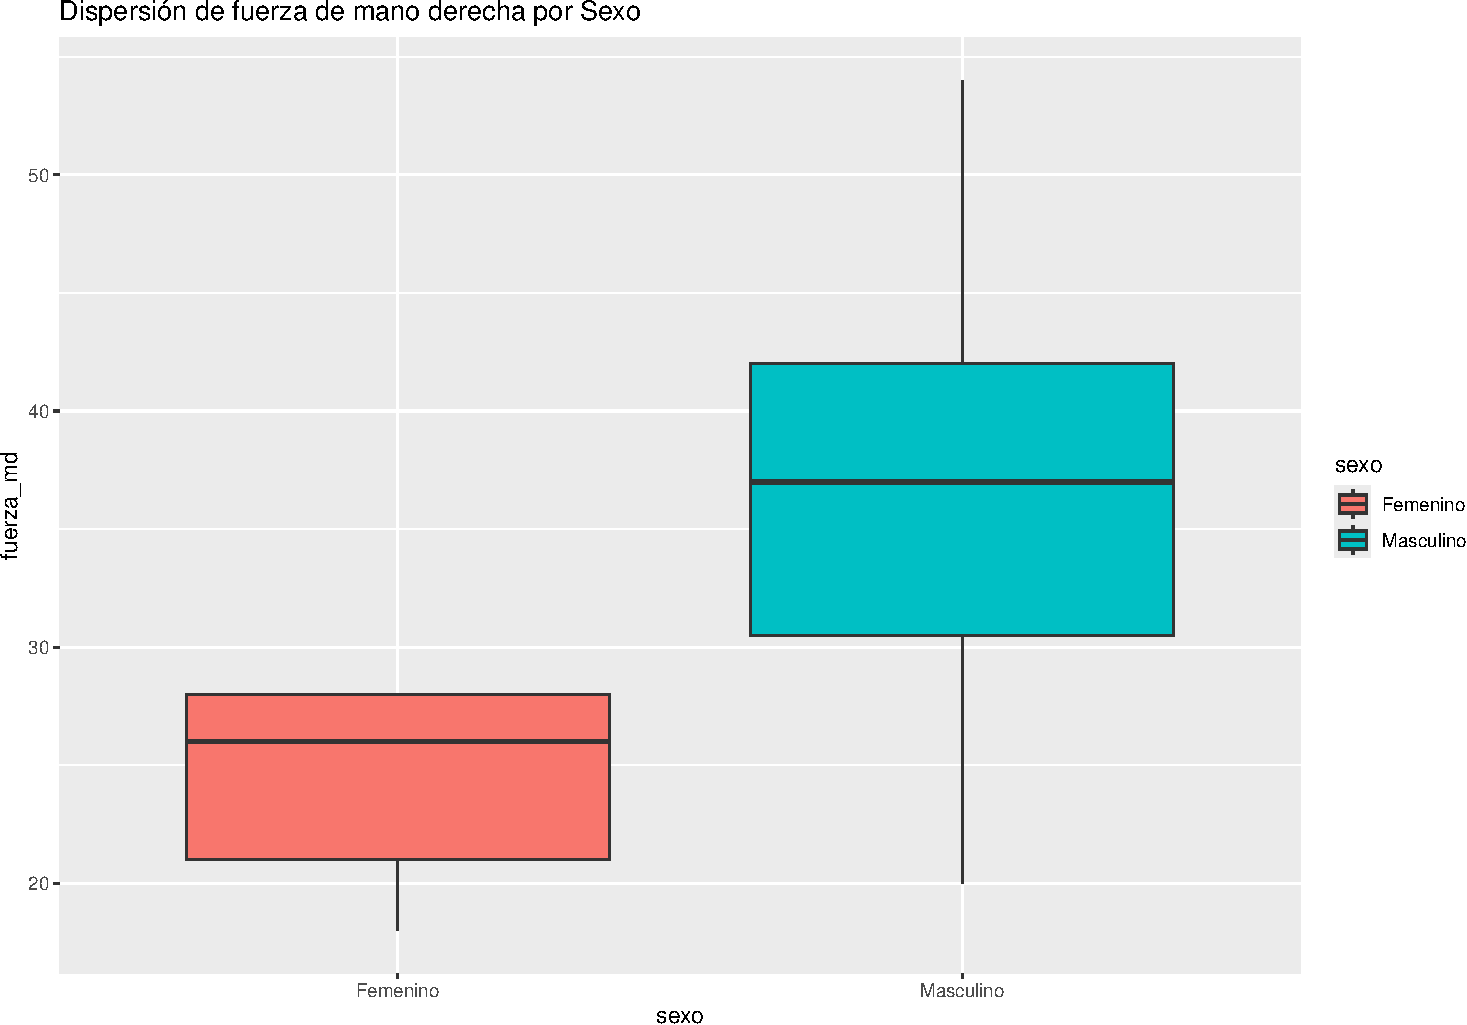
\includegraphics[keepaspectratio]{IntervalosHipotesis_files/figure-beamer/unnamed-chunk-8-1.pdf}}
\end{frame}

\begin{frame}{Conclusiones}
\phantomsection\label{conclusiones}
Se sospecha que:

\begin{itemize}
\item
  Hay diferencia en los promedios, dado que en el boxplot la caja de los
  hombres está mas arriba.
\item
  Las varianzas son distintas, lo cual se evidencia porque la caja de
  los hombres es más larga que la de las mujeres.
\end{itemize}
\end{frame}

\begin{frame}[fragile]{Estadísticas por \texttt{sexo}}
\phantomsection\label{estaduxedsticas-por-sexo}
Calculemos ahora la media, la varianza y el error estándar de la media,
desagregado por sexo.

\begin{figure*}

\begin{Shaded}
\begin{Highlighting}[]
\NormalTok{df}\SpecialCharTok{|\textgreater{}}\FunctionTok{group\_by}\NormalTok{(sexo)}\SpecialCharTok{|\textgreater{}}\FunctionTok{summarise}\NormalTok{(}\AttributeTok{N=}\FunctionTok{n}\NormalTok{(),}\AttributeTok{Media=}\FunctionTok{mean}\NormalTok{(fuerza\_md),}\AttributeTok{Var=}\FunctionTok{var}\NormalTok{(fuerza\_md))  }
\end{Highlighting}
\end{Shaded}

\begin{verbatim}
# A tibble: 2 x 4
  sexo          N  Media    Var
  <fct>     <int>  <dbl>  <dbl>
1 Femenino     11 24.364 14.255
2 Masculino    26 37.154 71.735
\end{verbatim}

\end{figure*}%
\end{frame}

\begin{frame}[fragile]{Error estándar de la media}
\phantomsection\label{error-estuxe1ndar-de-la-media}
Si no tenemos una función en el paquete base, la escribimos

\begin{figure*}

\begin{Shaded}
\begin{Highlighting}[]
\NormalTok{eemedia}\OtherTok{=}\ControlFlowTok{function}\NormalTok{(x)\{}
  \FunctionTok{sd}\NormalTok{(x,}\AttributeTok{na.rm =} \ConstantTok{TRUE}\NormalTok{)}\SpecialCharTok{/}\FunctionTok{sqrt}\NormalTok{(}\FunctionTok{length}\NormalTok{(}\FunctionTok{na.omit}\NormalTok{(x))) }
\NormalTok{\}}
\end{Highlighting}
\end{Shaded}

\end{figure*}%

\begin{figure*}

\begin{Shaded}
\begin{Highlighting}[]
\NormalTok{df}\SpecialCharTok{|\textgreater{}}\FunctionTok{group\_by}\NormalTok{(sexo)}\SpecialCharTok{|\textgreater{}}\FunctionTok{summarise}\NormalTok{(}\AttributeTok{N=}\FunctionTok{n}\NormalTok{(),}\AttributeTok{Media=}\FunctionTok{mean}\NormalTok{(fuerza\_md),}\AttributeTok{Var=}\FunctionTok{var}\NormalTok{(fuerza\_md),}\AttributeTok{Ee=}\FunctionTok{eemedia}\NormalTok{(fuerza\_md))  }
\end{Highlighting}
\end{Shaded}

\begin{verbatim}
# A tibble: 2 x 5
  sexo          N  Media    Var     Ee
  <fct>     <int>  <dbl>  <dbl>  <dbl>
1 Femenino     11 24.364 14.255 1.1384
2 Masculino    26 37.154 71.735 1.6610
\end{verbatim}

\end{figure*}%
\end{frame}

\begin{frame}[fragile]{Error estándar de la media II}
\phantomsection\label{error-estuxe1ndar-de-la-media-ii}
Sin usar la función

\begin{figure*}

\begin{Shaded}
\begin{Highlighting}[]
\NormalTok{df}\SpecialCharTok{|\textgreater{}}\FunctionTok{group\_by}\NormalTok{(sexo)}\SpecialCharTok{|\textgreater{}}\FunctionTok{summarise}\NormalTok{(}\AttributeTok{N=}\FunctionTok{n}\NormalTok{(),}\AttributeTok{Media=}\FunctionTok{mean}\NormalTok{(fuerza\_md),}\AttributeTok{Sd=}\FunctionTok{sd}\NormalTok{(fuerza\_md)) }\SpecialCharTok{|\textgreater{}} \FunctionTok{mutate}\NormalTok{(}\AttributeTok{ee=}\NormalTok{Sd}\SpecialCharTok{/}\FunctionTok{sqrt}\NormalTok{(N))   }
\end{Highlighting}
\end{Shaded}

\begin{verbatim}
# A tibble: 2 x 5
  sexo          N  Media     Sd     ee
  <fct>     <int>  <dbl>  <dbl>  <dbl>
1 Femenino     11 24.364 3.7755 1.1384
2 Masculino    26 37.154 8.4697 1.6610
\end{verbatim}

\end{figure*}%
\end{frame}

\section{Hipótesis sobre igualdad de
varianzas.}\label{hipuxf3tesis-sobre-igualdad-de-varianzas.}

\begin{frame}[fragile]{Prueba de igualdad de varianzas}
\phantomsection\label{prueba-de-igualdad-de-varianzas}
\begin{tcolorbox}[enhanced jigsaw, colbacktitle=quarto-callout-warning-color!10!white, coltitle=black, title=\textcolor{quarto-callout-warning-color}{\faExclamationTriangle}\hspace{0.5em}{Warning}, breakable, bottomrule=.15mm, colback=white, toprule=.15mm, bottomtitle=1mm, toptitle=1mm, titlerule=0mm, rightrule=.15mm, arc=.35mm, leftrule=.75mm, colframe=quarto-callout-warning-color-frame, opacitybacktitle=0.6, left=2mm, opacityback=0]

Antes de probar la hipótesis con respecto a la media, debemos probar si
se cumple el supuesto de varianzas iguales.

\end{tcolorbox}

Probaremos la hipótesis \[H_0:\sigma^2_m=\sigma^2_f\] con una prueba
\(F\), implementada en la función \texttt{var.test}.
\end{frame}

\begin{frame}[fragile]{Uso de \texttt{var.test}}
\phantomsection\label{uso-de-var.test}
\begin{figure*}

\begin{Shaded}
\begin{Highlighting}[]
\NormalTok{df }\SpecialCharTok{|\textgreater{}}\FunctionTok{with}\NormalTok{(}\FunctionTok{var.test}\NormalTok{(fuerza\_md}\SpecialCharTok{\textasciitilde{}}\NormalTok{sexo)) }
\end{Highlighting}
\end{Shaded}

\begin{verbatim}

    F test to compare two variances

data:  fuerza_md by sexo
F = 0.19871, num df = 10, denom df = 25, p-value = 0.01098
alternative hypothesis: true ratio of variances is not equal to 1
95 percent confidence interval:
 0.07603316 0.66659195
sample estimates:
ratio of variances 
         0.1987101 
\end{verbatim}

\end{figure*}%

\begin{figure*}

\begin{Shaded}
\begin{Highlighting}[]
\NormalTok{resultados\_f }\OtherTok{\textless{}{-}}\NormalTok{ df }\SpecialCharTok{|\textgreater{}}\FunctionTok{with}\NormalTok{(}\FunctionTok{var.test}\NormalTok{(fuerza\_md}\SpecialCharTok{\textasciitilde{}}\NormalTok{sexo))}\SpecialCharTok{|\textgreater{}}\FunctionTok{tidy}\NormalTok{()}
\end{Highlighting}
\end{Shaded}

\end{figure*}%

\begin{figure*}

\begin{Shaded}
\begin{Highlighting}[]
\FunctionTok{print}\NormalTok{(resultados\_f ) }
\end{Highlighting}
\end{Shaded}

\begin{verbatim}
# A tibble: 1 x 9
  estimate num.df den.df statistic  p.value conf.low conf.high method           
     <dbl>  <int>  <int>     <dbl>    <dbl>    <dbl>     <dbl> <chr>            
1  0.19871     10     25   0.19871 0.010982 0.076033   0.66659 F test to compar~
# i 1 more variable: alternative <chr>
\end{verbatim}

\end{figure*}%
\end{frame}

\section{Hipótesis sobre igualdad de medias, varianzas
distintas}\label{hipuxf3tesis-sobre-igualdad-de-medias-varianzas-distintas}

\begin{frame}[fragile]{Prueba de la hipótesis}
\phantomsection\label{prueba-de-la-hipuxf3tesis}
Prueba T de Welch \texttt{Var.equal\ =\ FALSE} por defecto en R

Probaremos la hipótesis \[
H_0: \mu_m=\mu_f \\
H_1: \mu_m>\mu_f\]

\begin{figure*}

\begin{Shaded}
\begin{Highlighting}[]
\NormalTok{resultados\_t }\OtherTok{\textless{}{-}}\NormalTok{ df }\SpecialCharTok{|\textgreater{}}\FunctionTok{with}\NormalTok{(}\FunctionTok{t.test}\NormalTok{(fuerza\_md}\SpecialCharTok{\textasciitilde{}}\NormalTok{sexo,}\AttributeTok{alternative=}\StringTok{\textquotesingle{}greater\textquotesingle{}}\NormalTok{))}\SpecialCharTok{|\textgreater{}}\FunctionTok{tidy}\NormalTok{()}
\FunctionTok{print}\NormalTok{(resultados\_t)}
\end{Highlighting}
\end{Shaded}

\begin{verbatim}
# A tibble: 1 x 10
  estimate estimate1 estimate2 statistic p.value parameter conf.low conf.high
     <dbl>     <dbl>     <dbl>     <dbl>   <dbl>     <dbl>    <dbl>     <dbl>
1  -12.790    24.364    37.154   -6.3516  1.0000    34.804  -16.193       Inf
# i 2 more variables: method <chr>, alternative <chr>
\end{verbatim}

\end{figure*}%
\end{frame}

\begin{frame}{¿Qué se concluye?}
\phantomsection\label{quuxe9-se-concluye}
\begin{tcolorbox}[enhanced jigsaw, colbacktitle=quarto-callout-caution-color!10!white, coltitle=black, title=\textcolor{quarto-callout-caution-color}{\faFire}\hspace{0.5em}{Caution}, breakable, bottomrule=.15mm, colback=white, toprule=.15mm, bottomtitle=1mm, toptitle=1mm, titlerule=0mm, rightrule=.15mm, arc=.35mm, leftrule=.75mm, colframe=quarto-callout-caution-color-frame, opacitybacktitle=0.6, left=2mm, opacityback=0]

No se rechaza la hipótesis nula porque el valor p es mayor que 0.05

\end{tcolorbox}

\begin{tcolorbox}[enhanced jigsaw, colbacktitle=quarto-callout-warning-color!10!white, coltitle=black, title=\textcolor{quarto-callout-warning-color}{\faExclamationTriangle}\hspace{0.5em}{Warning}, breakable, bottomrule=.15mm, colback=white, toprule=.15mm, bottomtitle=1mm, toptitle=1mm, titlerule=0mm, rightrule=.15mm, arc=.35mm, leftrule=.75mm, colframe=quarto-callout-warning-color-frame, opacitybacktitle=0.6, left=2mm, opacityback=0]

La conclusión anterior no es correcta, porque la diferencia de media se
está calculando al revés

\end{tcolorbox}
\end{frame}

\section{Nivel de referencia de un
factor.}\label{nivel-de-referencia-de-un-factor.}

\begin{frame}[fragile]{Nivel de referencia}
\phantomsection\label{nivel-de-referencia}
\begin{figure*}

\begin{Shaded}
\begin{Highlighting}[]
\NormalTok{df}\SpecialCharTok{$}\NormalTok{sexo}\OtherTok{=}\FunctionTok{factor}\NormalTok{(df}\SpecialCharTok{$}\NormalTok{sexo)}
\FunctionTok{levels}\NormalTok{(df}\SpecialCharTok{$}\NormalTok{sexo) }
\end{Highlighting}
\end{Shaded}

\begin{verbatim}
[1] "Femenino"  "Masculino"
\end{verbatim}

\end{figure*}%

\begin{figure*}

\begin{Shaded}
\begin{Highlighting}[]
\NormalTok{df}\SpecialCharTok{$}\NormalTok{sexo}\OtherTok{=}\FunctionTok{relevel}\NormalTok{(df}\SpecialCharTok{$}\NormalTok{sexo,}\AttributeTok{ref=}\StringTok{"Masculino"}\NormalTok{) }
\FunctionTok{levels}\NormalTok{(df}\SpecialCharTok{$}\NormalTok{sexo) }
\end{Highlighting}
\end{Shaded}

\begin{verbatim}
[1] "Masculino" "Femenino" 
\end{verbatim}

\end{figure*}%
\end{frame}

\begin{frame}[fragile]{Repetimos la prueba}
\phantomsection\label{repetimos-la-prueba}
\begin{figure*}

\begin{Shaded}
\begin{Highlighting}[]
\NormalTok{resultados\_t }\OtherTok{\textless{}{-}}\NormalTok{ df }\SpecialCharTok{|\textgreater{}}\FunctionTok{with}\NormalTok{(}\FunctionTok{t.test}\NormalTok{(fuerza\_md}\SpecialCharTok{\textasciitilde{}}\NormalTok{sexo,}\AttributeTok{alternative=}\StringTok{\textquotesingle{}greater\textquotesingle{}}\NormalTok{))}\SpecialCharTok{|\textgreater{}}\FunctionTok{tidy}\NormalTok{()}
\FunctionTok{print}\NormalTok{(resultados\_t)}
\end{Highlighting}
\end{Shaded}

\begin{verbatim}
# A tibble: 1 x 10
  estimate estimate1 estimate2 statistic    p.value parameter conf.low conf.high
     <dbl>     <dbl>     <dbl>     <dbl>      <dbl>     <dbl>    <dbl>     <dbl>
1   12.790    37.154    24.364    6.3516  1.3650e-7    34.804   9.3874       Inf
# i 2 more variables: method <chr>, alternative <chr>
\end{verbatim}

\end{figure*}%
\end{frame}

\section{Hipótesis sobre la diferencia de medias, varianzas
iguales.}\label{hipuxf3tesis-sobre-la-diferencia-de-medias-varianzas-iguales.}

\begin{frame}{Pregunta a responder}
\phantomsection\label{pregunta-a-responder-1}
\begin{tcolorbox}[enhanced jigsaw, colbacktitle=quarto-callout-important-color!10!white, coltitle=black, title=\textcolor{quarto-callout-important-color}{\faExclamation}\hspace{0.5em}{Important}, breakable, bottomrule=.15mm, colback=white, toprule=.15mm, bottomtitle=1mm, toptitle=1mm, titlerule=0mm, rightrule=.15mm, arc=.35mm, leftrule=.75mm, colframe=quarto-callout-important-color-frame, opacitybacktitle=0.6, left=2mm, opacityback=0]

Hipótesis: La masa muscular promedio es mayor en hombres que en mujeres.

\end{tcolorbox}
\end{frame}

\begin{frame}[fragile]{Visualización previa}
\phantomsection\label{visualizaciuxf3n-previa-1}
\begin{Shaded}
\begin{Highlighting}[]
\FunctionTok{library}\NormalTok{(tidyverse)}
\FunctionTok{library}\NormalTok{(broom)}
\NormalTok{df }\SpecialCharTok{|\textgreater{}} 
  \FunctionTok{ggplot}\NormalTok{(}\FunctionTok{aes}\NormalTok{(}\AttributeTok{x =}\NormalTok{ sexo, }\AttributeTok{y =}\NormalTok{ masa\_muscular, }\AttributeTok{fill =}\NormalTok{ sexo)) }\SpecialCharTok{+}
  \FunctionTok{geom\_boxplot}\NormalTok{() }\SpecialCharTok{+}
  \FunctionTok{labs}\NormalTok{(}\AttributeTok{title =} \StringTok{"Dispersión de Masa Muscular por Sexo"}\NormalTok{)}
\end{Highlighting}
\end{Shaded}

\pandocbounded{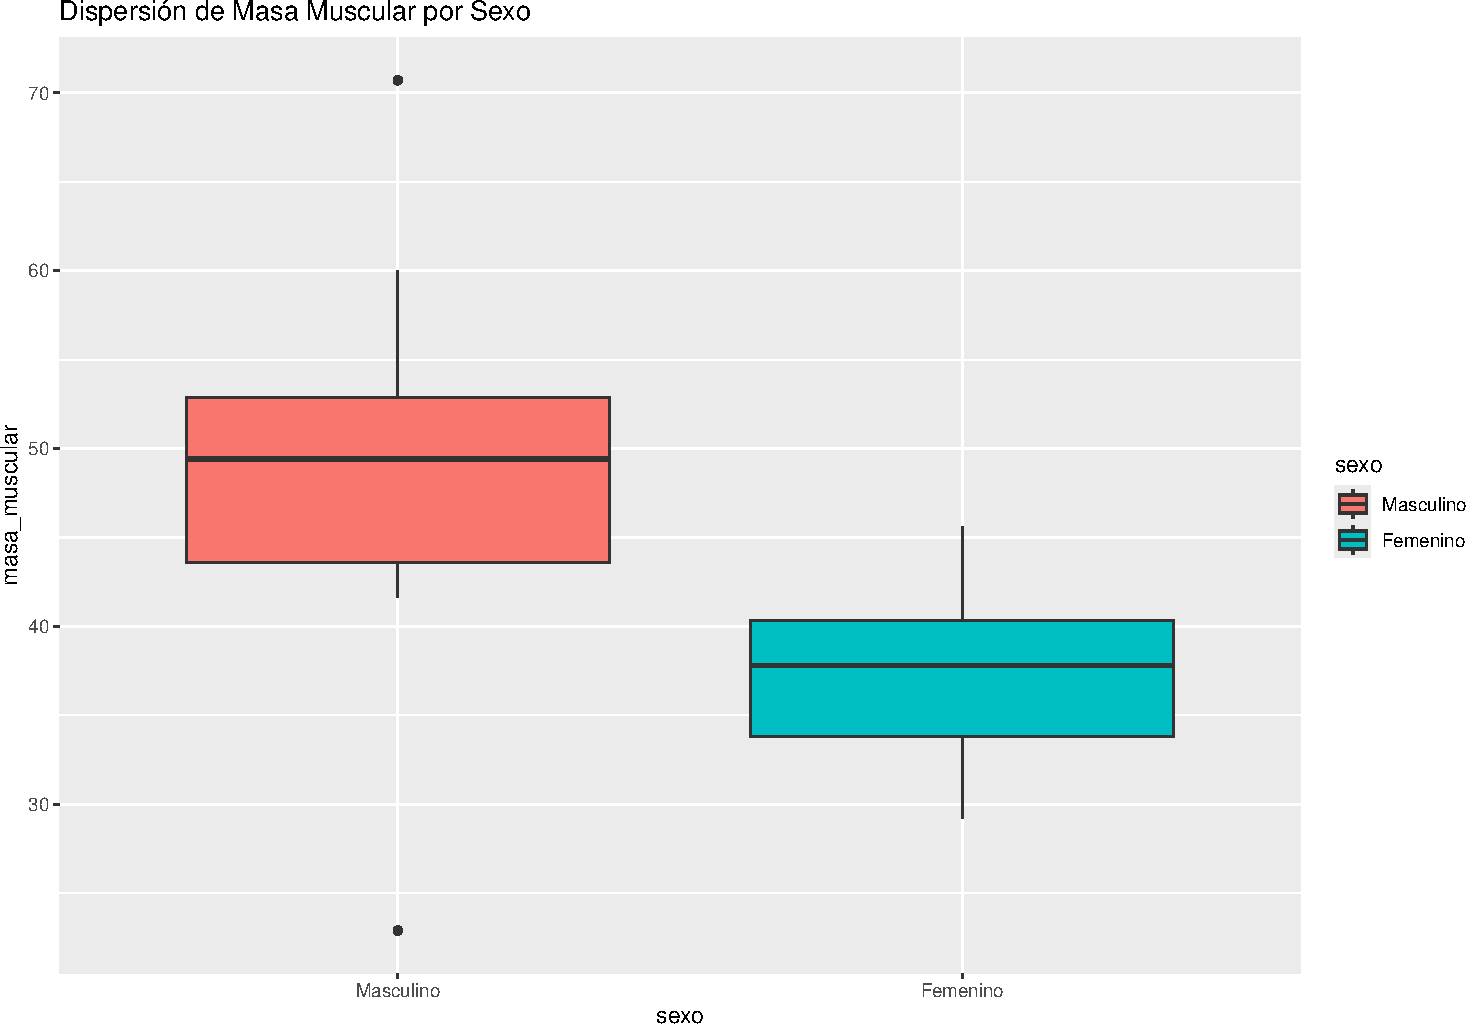
\includegraphics[keepaspectratio]{IntervalosHipotesis_files/figure-beamer/unnamed-chunk-20-1.pdf}}
\end{frame}

\begin{frame}{Conclusiones}
\phantomsection\label{conclusiones-1}
Se sospecha que:

\begin{itemize}
\item
  Hay diferencia en los promedios, dado que en el boxplot la caja de los
  hombres está mas arriba.
\item
  Las varianzas son distintas, lo cual se evidencia porque la caja de
  los hombres es más larga que la de las mujeres.
\end{itemize}
\end{frame}

\begin{frame}[fragile]{Estadísticas por \texttt{sexo}}
\phantomsection\label{estaduxedsticas-por-sexo-1}
Calculemos ahora la media, la varianza y el error estándar de la media,
desagregado por sexo.

\begin{figure*}

\begin{Shaded}
\begin{Highlighting}[]
\NormalTok{df}\SpecialCharTok{|\textgreater{}}\FunctionTok{group\_by}\NormalTok{(sexo)}\SpecialCharTok{|\textgreater{}}\FunctionTok{summarise}\NormalTok{(}\AttributeTok{N=}\FunctionTok{n}\NormalTok{(),}\AttributeTok{Media=}\FunctionTok{mean}\NormalTok{(masa\_muscular),}\AttributeTok{Var=}\FunctionTok{var}\NormalTok{(masa\_muscular))  }
\end{Highlighting}
\end{Shaded}

\begin{verbatim}
# A tibble: 2 x 4
  sexo          N  Media    Var
  <fct>     <int>  <dbl>  <dbl>
1 Masculino    26 48.785 78.011
2 Femenino     11 37.368 26.175
\end{verbatim}

\end{figure*}%
\end{frame}

\begin{frame}[fragile]{Error estándar de la media}
\phantomsection\label{error-estuxe1ndar-de-la-media-1}
Si no tenemos una función en el paquete base, la escribimos

\begin{figure*}

\begin{Shaded}
\begin{Highlighting}[]
\NormalTok{eemedia}\OtherTok{=}\ControlFlowTok{function}\NormalTok{(x)\{}
  \FunctionTok{sd}\NormalTok{(x,}\AttributeTok{na.rm =} \ConstantTok{TRUE}\NormalTok{)}\SpecialCharTok{/}\FunctionTok{length}\NormalTok{(}\FunctionTok{na.omit}\NormalTok{(x)) }
\NormalTok{\}}
\end{Highlighting}
\end{Shaded}

\end{figure*}%

\begin{figure*}

\begin{Shaded}
\begin{Highlighting}[]
\NormalTok{df}\SpecialCharTok{|\textgreater{}}\FunctionTok{group\_by}\NormalTok{(sexo)}\SpecialCharTok{|\textgreater{}}\FunctionTok{summarise}\NormalTok{(}\AttributeTok{N=}\FunctionTok{n}\NormalTok{(),}\AttributeTok{Media=}\FunctionTok{mean}\NormalTok{(masa\_muscular),}\AttributeTok{Var=}\FunctionTok{var}\NormalTok{(masa\_muscular),}\AttributeTok{Ee=}\FunctionTok{eemedia}\NormalTok{(masa\_muscular))  }
\end{Highlighting}
\end{Shaded}

\begin{verbatim}
# A tibble: 2 x 5
  sexo          N  Media    Var      Ee
  <fct>     <int>  <dbl>  <dbl>   <dbl>
1 Masculino    26 48.785 78.011 0.33971
2 Femenino     11 37.368 26.175 0.46511
\end{verbatim}

\end{figure*}%
\end{frame}

\begin{frame}[fragile]{Prueba de igualdad de varianzas}
\phantomsection\label{prueba-de-igualdad-de-varianzas-1}
\begin{tcolorbox}[enhanced jigsaw, colbacktitle=quarto-callout-warning-color!10!white, coltitle=black, title=\textcolor{quarto-callout-warning-color}{\faExclamationTriangle}\hspace{0.5em}{Warning}, breakable, bottomrule=.15mm, colback=white, toprule=.15mm, bottomtitle=1mm, toptitle=1mm, titlerule=0mm, rightrule=.15mm, arc=.35mm, leftrule=.75mm, colframe=quarto-callout-warning-color-frame, opacitybacktitle=0.6, left=2mm, opacityback=0]

Antes de probar la hipótesis con respecto a la media, debemos probar si
se cumple el supuesto de varianzas iguales.

\end{tcolorbox}

Probaremos la hipótesis \[H_0:\sigma^2_m=\sigma^2_f\] con una prueba
\(F\), implementada en la función \texttt{var.test}.
\end{frame}

\begin{frame}[fragile]{Uso de \texttt{var.test}}
\phantomsection\label{uso-de-var.test-1}
\begin{figure*}

\begin{Shaded}
\begin{Highlighting}[]
\NormalTok{resultados\_f }\OtherTok{\textless{}{-}}\NormalTok{ df }\SpecialCharTok{|\textgreater{}}\FunctionTok{with}\NormalTok{(}\FunctionTok{var.test}\NormalTok{(masa\_muscular}\SpecialCharTok{\textasciitilde{}}\NormalTok{sexo))}\SpecialCharTok{|\textgreater{}}\FunctionTok{tidy}\NormalTok{()}
\end{Highlighting}
\end{Shaded}

\end{figure*}%

\begin{figure*}

\begin{Shaded}
\begin{Highlighting}[]
\FunctionTok{print}\NormalTok{(resultados\_f ) }
\end{Highlighting}
\end{Shaded}

\begin{verbatim}
# A tibble: 1 x 9
  estimate num.df den.df statistic  p.value conf.low conf.high method           
     <dbl>  <int>  <int>     <dbl>    <dbl>    <dbl>     <dbl> <chr>            
1   2.9803     25     10    2.9803 0.074964  0.88843    7.7890 F test to compar~
# i 1 more variable: alternative <chr>
\end{verbatim}

\end{figure*}%
\end{frame}

\begin{frame}{Conclusión}
\phantomsection\label{conclusiuxf3n}
\begin{tcolorbox}[enhanced jigsaw, colbacktitle=quarto-callout-note-color!10!white, coltitle=black, title=\textcolor{quarto-callout-note-color}{\faInfo}\hspace{0.5em}{Note}, breakable, bottomrule=.15mm, colback=white, toprule=.15mm, bottomtitle=1mm, toptitle=1mm, titlerule=0mm, rightrule=.15mm, arc=.35mm, leftrule=.75mm, colframe=quarto-callout-note-color-frame, opacitybacktitle=0.6, left=2mm, opacityback=0]

a un nivel de significancia del 5\% no se rechaza la hipótesis de
igualdad de varianzas. Asumimos varianzas poblacionales iguales.

\end{tcolorbox}
\end{frame}

\begin{frame}[fragile]{Prueba de la hipótesis}
\phantomsection\label{prueba-de-la-hipuxf3tesis-1}
Prueba T con varianzas iguales, debemos indicar:
\texttt{Var.equal\ =TRUE} en la función \texttt{t.test}

\begin{figure*}

\begin{Shaded}
\begin{Highlighting}[]
\NormalTok{prueba\_t}\OtherTok{\textless{}{-}}\NormalTok{ df}\SpecialCharTok{|\textgreater{}}\FunctionTok{with}\NormalTok{(}\FunctionTok{t.test}\NormalTok{(masa\_muscular }\SpecialCharTok{\textasciitilde{}}\NormalTok{ sexo, }\AttributeTok{var.equal =} \ConstantTok{TRUE}\NormalTok{))}\SpecialCharTok{|\textgreater{}}\FunctionTok{tidy}\NormalTok{()}
\FunctionTok{print}\NormalTok{(prueba\_t) }
\end{Highlighting}
\end{Shaded}

\begin{verbatim}
# A tibble: 1 x 10
  estimate estimate1 estimate2 statistic    p.value parameter conf.low conf.high
     <dbl>     <dbl>     <dbl>     <dbl>      <dbl>     <dbl>    <dbl>     <dbl>
1   11.416    48.785    37.368    3.9926 0.00031898        35   5.6115    17.221
# i 2 more variables: method <chr>, alternative <chr>
\end{verbatim}

\end{figure*}%
\end{frame}

\begin{frame}{Explicación al resultado}
\phantomsection\label{explicaciuxf3n-al-resultado}
Masa Muscular por Sexo: Fisiológicamente, los hombres suelen tener no
solo una media de masa muscular más alta, sino también una mayor
variabilidad (dispersión) debido a factores hormonales y de actividad
física diversa.
\end{frame}

\section{Prueba T pareada}\label{prueba-t-pareada}

\begin{frame}{Pregunta a responder}
\phantomsection\label{pregunta-a-responder-2}
\begin{tcolorbox}[enhanced jigsaw, colbacktitle=quarto-callout-important-color!10!white, coltitle=black, title=\textcolor{quarto-callout-important-color}{\faExclamation}\hspace{0.5em}{Important}, breakable, bottomrule=.15mm, colback=white, toprule=.15mm, bottomtitle=1mm, toptitle=1mm, titlerule=0mm, rightrule=.15mm, arc=.35mm, leftrule=.75mm, colframe=quarto-callout-important-color-frame, opacitybacktitle=0.6, left=2mm, opacityback=0]

¿La fuerza prensil promedio de la mano derecha es igual a la de la mazo
izquierda?

\end{tcolorbox}
\end{frame}

\begin{frame}{Exploración gráfica}
\phantomsection\label{exploraciuxf3n-gruxe1fica}
\begin{itemize}
\item
  Graficamos los datos de fuerza prensil buscando visualizar la relación
  entre manos.
\item
  Graficamos los datos de fuerza prensil buscando visualizar la relación
  entre manos y diferenciando por sexo.
\end{itemize}
\end{frame}

\begin{frame}[fragile]{Gráfico de dispersaión}
\phantomsection\label{gruxe1fico-de-dispersaiuxf3n}
\begin{Shaded}
\begin{Highlighting}[]
\FunctionTok{ggplot}\NormalTok{(df,}\FunctionTok{aes}\NormalTok{(}\AttributeTok{x=}\NormalTok{fuerza\_md, }\AttributeTok{y=}\NormalTok{fuerza\_mi)) }\SpecialCharTok{+} \FunctionTok{geom\_point}\NormalTok{()}
\end{Highlighting}
\end{Shaded}

\begin{figure*}[H]

\pandocbounded{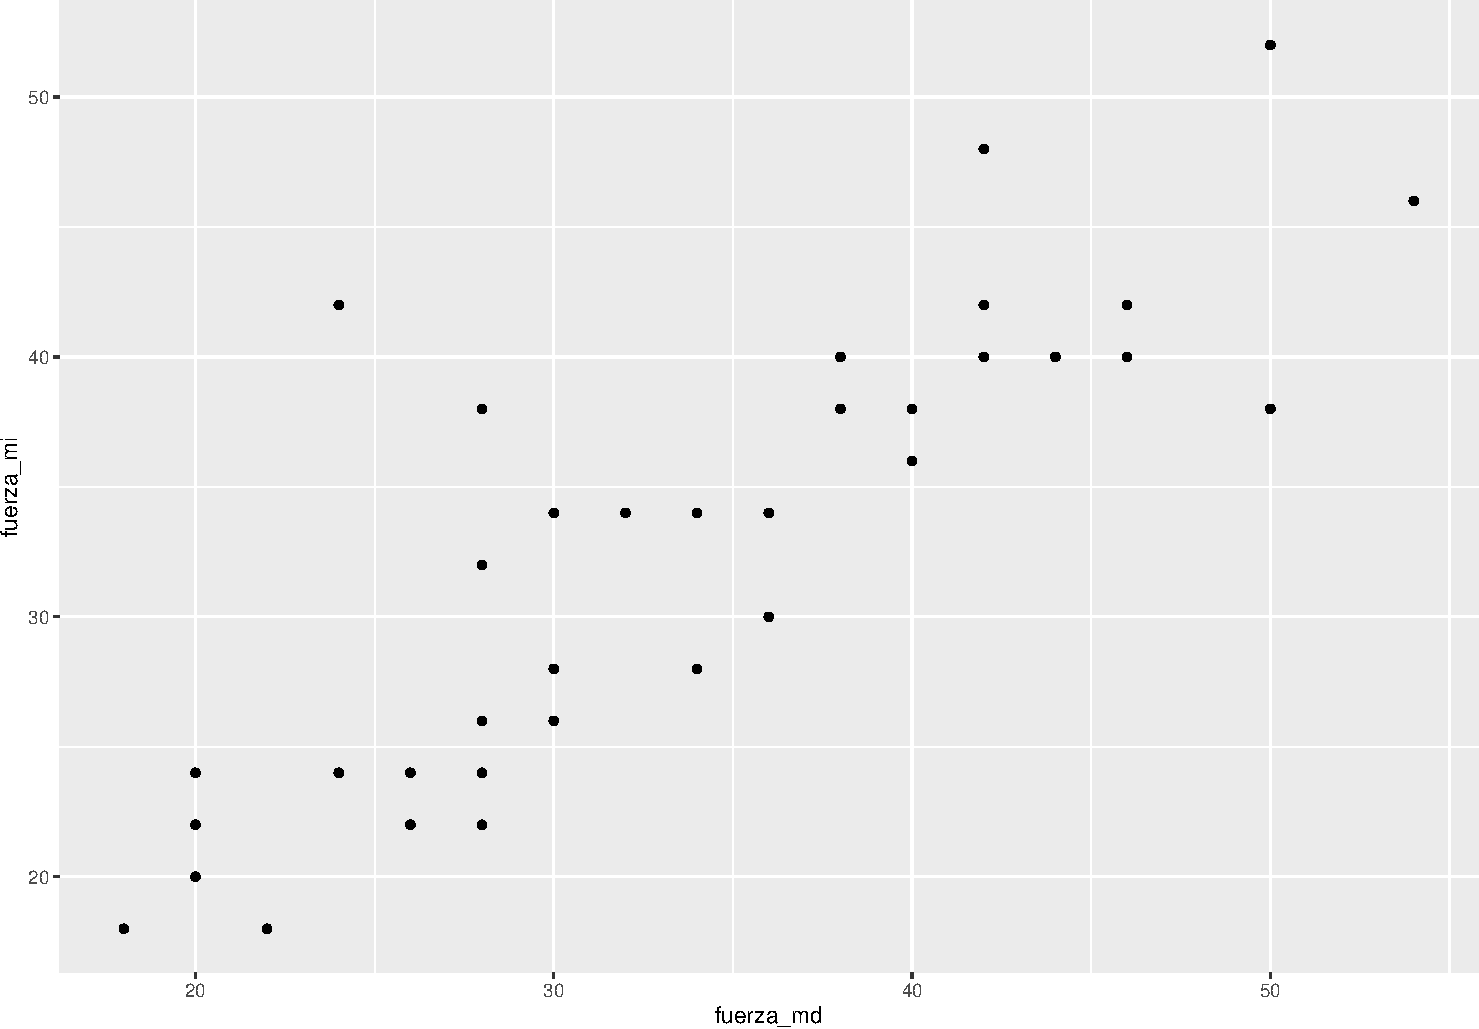
\includegraphics[keepaspectratio]{IntervalosHipotesis_files/figure-beamer/unnamed-chunk-27-1.pdf}}

\end{figure*}
\end{frame}

\begin{frame}[fragile]{Exploración gráfica (diferenciamos por sexo)}
\phantomsection\label{exploraciuxf3n-gruxe1fica-diferenciamos-por-sexo}
\begin{Shaded}
\begin{Highlighting}[]
\FunctionTok{ggplot}\NormalTok{(df,}\FunctionTok{aes}\NormalTok{(}\AttributeTok{x=}\NormalTok{fuerza\_md, }\AttributeTok{y=}\NormalTok{fuerza\_mi,}\AttributeTok{col=}\NormalTok{sexo)) }\SpecialCharTok{+} \FunctionTok{geom\_point}\NormalTok{()}
\end{Highlighting}
\end{Shaded}

\begin{figure*}[H]

\pandocbounded{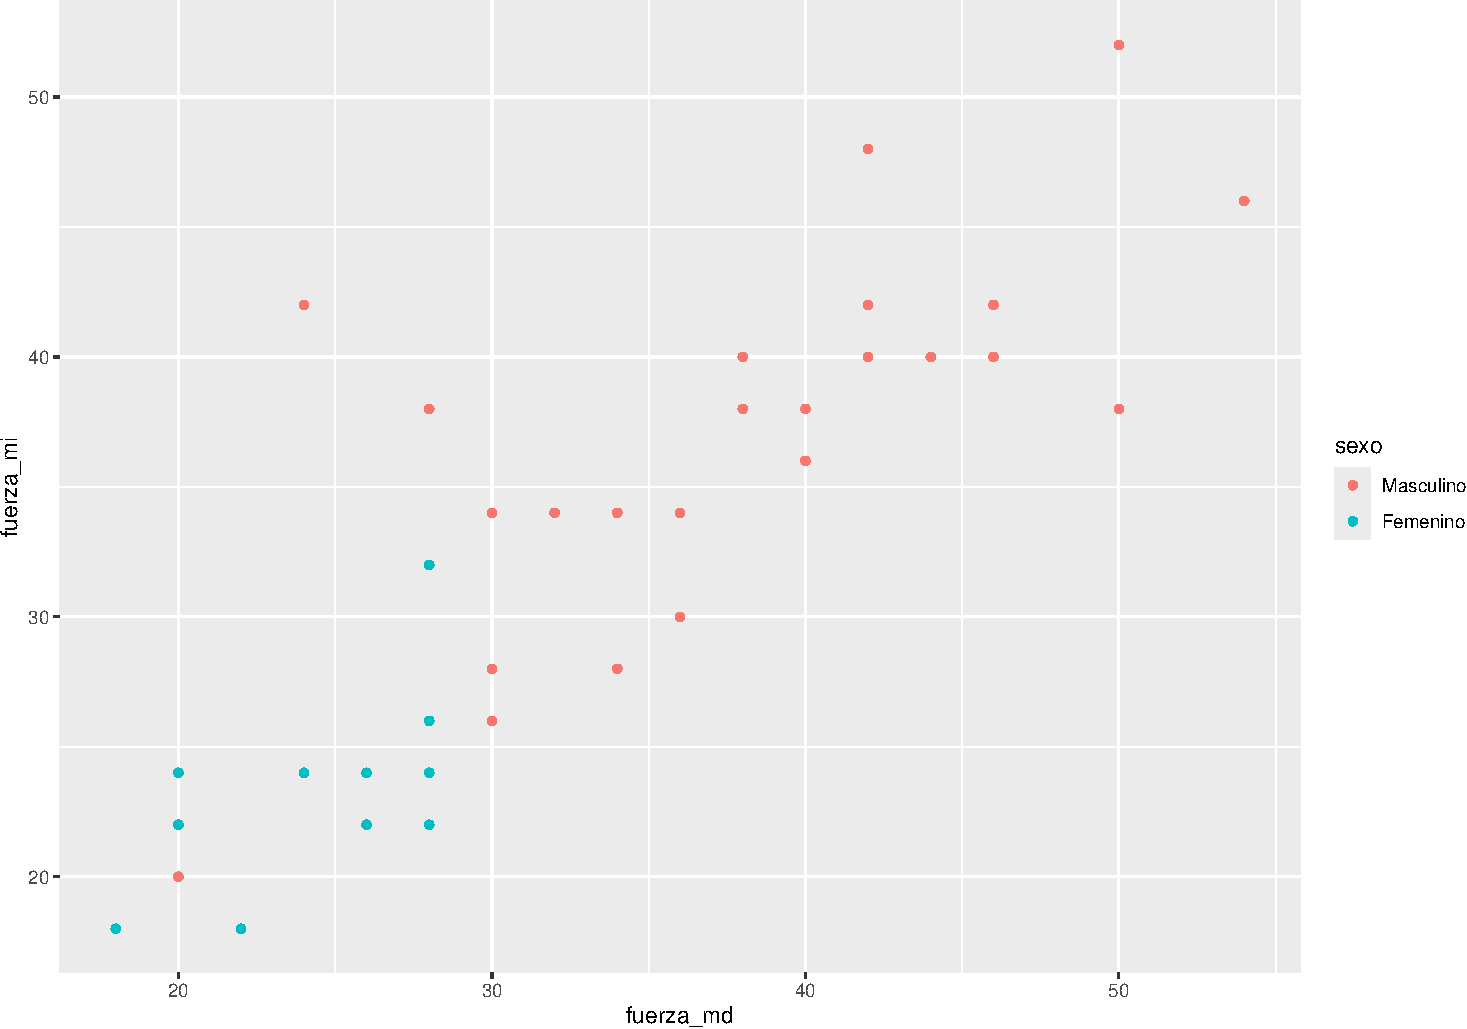
\includegraphics[keepaspectratio]{IntervalosHipotesis_files/figure-beamer/unnamed-chunk-28-1.pdf}}

\end{figure*}
\end{frame}

\begin{frame}{Ejercicio}
\phantomsection\label{ejercicio}
\begin{figure*}[H]

\pandocbounded{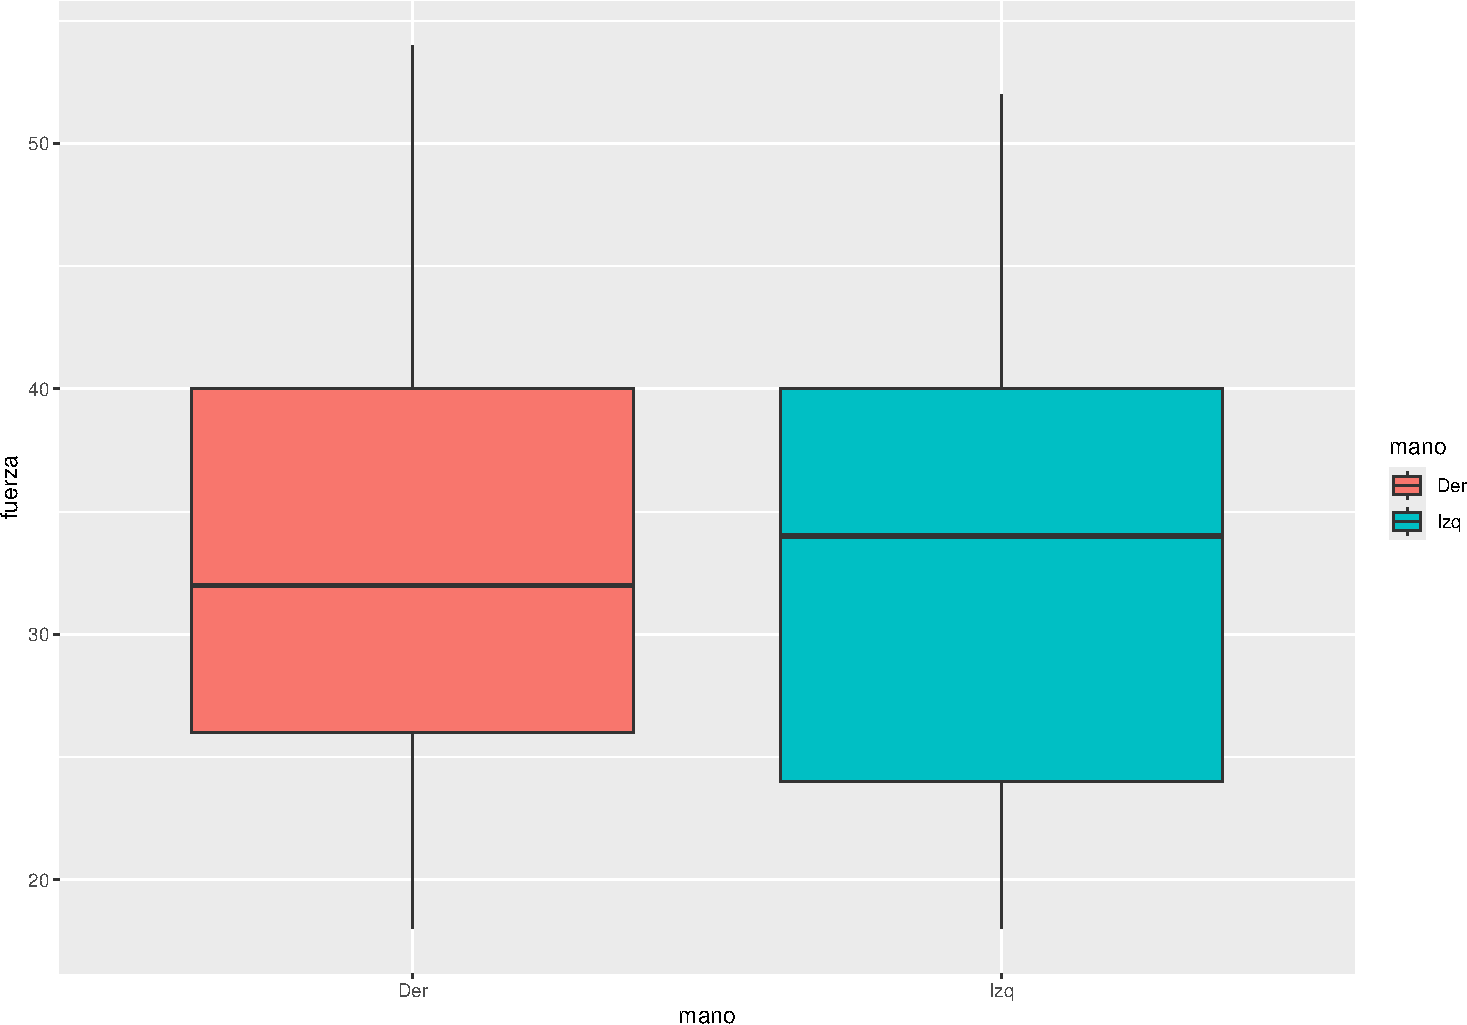
\includegraphics[keepaspectratio]{IntervalosHipotesis_files/figure-beamer/unnamed-chunk-29-1.pdf}}

\end{figure*}
\end{frame}

\begin{frame}[fragile]{Descriptivas}
\phantomsection\label{descriptivas}
\begin{figure*}

\begin{Shaded}
\begin{Highlighting}[]
\NormalTok{fuerza}\SpecialCharTok{|\textgreater{}}\FunctionTok{group\_by}\NormalTok{(mano)}\SpecialCharTok{|\textgreater{}}\FunctionTok{summarise}\NormalTok{(}\AttributeTok{n=}\FunctionTok{n}\NormalTok{(),}\AttributeTok{Media=}\FunctionTok{mean}\NormalTok{(fuerza),}\AttributeTok{Mediana=}\FunctionTok{median}\NormalTok{(fuerza),}\AttributeTok{Var=}\FunctionTok{var}\NormalTok{(fuerza))   }
\end{Highlighting}
\end{Shaded}

\begin{verbatim}
# A tibble: 2 x 5
  mano      n  Media Mediana    Var
  <fct> <int>  <dbl>   <int>  <dbl>
1 Der      37 33.351      32 88.901
2 Izq      37 32.432      34 80.030
\end{verbatim}

\begin{Shaded}
\begin{Highlighting}[]
\CommentTok{\#fuerza|\textgreater{}ggplot(aes(x=mano,y=fuerza,fill = mano))+geom\_boxplot()}
\end{Highlighting}
\end{Shaded}

\end{figure*}%
\end{frame}

\begin{frame}[fragile]{Estadísticas descriptivas}
\phantomsection\label{estaduxedsticas-descriptivas}
\begin{figure*}

\begin{Shaded}
\begin{Highlighting}[]
\NormalTok{df}\SpecialCharTok{|\textgreater{}}\FunctionTok{group\_by}\NormalTok{(sexo)}\SpecialCharTok{|\textgreater{}}\FunctionTok{summarise}\NormalTok{(}\AttributeTok{N=}\FunctionTok{n}\NormalTok{(),}\AttributeTok{MediaI=}\FunctionTok{mean}\NormalTok{(fuerza\_mi),}\AttributeTok{MediaD=}\FunctionTok{mean}\NormalTok{(fuerza\_md),}\AttributeTok{SdI=}\FunctionTok{sd}\NormalTok{(fuerza\_mi),}\AttributeTok{SdD=}\FunctionTok{sd}\NormalTok{(fuerza\_md))  }
\end{Highlighting}
\end{Shaded}

\begin{verbatim}
# A tibble: 2 x 6
  sexo          N MediaI MediaD    SdI    SdD
  <fct>     <int>  <dbl>  <dbl>  <dbl>  <dbl>
1 Masculino    26 36.308 37.154 7.5407 8.4697
2 Femenino     11 23.273 24.364 3.8234 3.7755
\end{verbatim}

\end{figure*}%
\end{frame}

\begin{frame}[fragile]{Prueba de la hipótesis}
\phantomsection\label{prueba-de-la-hipuxf3tesis-2}
\begin{figure*}

\begin{Shaded}
\begin{Highlighting}[]
\FunctionTok{library}\NormalTok{(broom)}
\FunctionTok{library}\NormalTok{(knitr) }

\NormalTok{resultados\_t }\OtherTok{\textless{}{-}}\NormalTok{ df }\SpecialCharTok{|\textgreater{}}
  \FunctionTok{filter}\NormalTok{(}\SpecialCharTok{!}\FunctionTok{is.na}\NormalTok{(fuerza\_md), }\SpecialCharTok{!}\FunctionTok{is.na}\NormalTok{(fuerza\_mi)) }\SpecialCharTok{|\textgreater{}}
  \FunctionTok{with}\NormalTok{(}\FunctionTok{t.test}\NormalTok{(fuerza\_md, fuerza\_mi, }\AttributeTok{paired =} \ConstantTok{TRUE}\NormalTok{)) }\SpecialCharTok{|\textgreater{}}
  \FunctionTok{tidy}\NormalTok{()}

\FunctionTok{print}\NormalTok{(resultados\_t)}
\end{Highlighting}
\end{Shaded}

\begin{verbatim}
# A tibble: 1 x 8
  estimate statistic p.value parameter conf.low conf.high method     alternative
     <dbl>     <dbl>   <dbl>     <dbl>    <dbl>     <dbl> <chr>      <chr>      
1  0.91892    1.0623 0.29519        36 -0.83549    2.6733 Paired t-~ two.sided  
\end{verbatim}

\end{figure*}%
\end{frame}

\begin{frame}[fragile]{II}
\phantomsection\label{ii}
\begin{Shaded}
\begin{Highlighting}[]
\FunctionTok{library}\NormalTok{(knitr)}
\FunctionTok{library}\NormalTok{(kableExtra) }\CommentTok{\# Este es el paquete clave}

\CommentTok{\# Presentación elegante para HTML}
\NormalTok{resultados\_t }\SpecialCharTok{|\textgreater{}}
  \FunctionTok{kable}\NormalTok{(}
    \AttributeTok{digits =} \DecValTok{4}\NormalTok{, }
    \AttributeTok{caption =} \StringTok{"Resultados de la Prueba t para Muestras Pareadas: Fuerza MD vs MI"}\NormalTok{,}
    \AttributeTok{col.names =} \FunctionTok{c}\NormalTok{(}\StringTok{"Estimación"}\NormalTok{, }\StringTok{"Estadístico t"}\NormalTok{, }\StringTok{"p{-}valor"}\NormalTok{, }\StringTok{"gl"}\NormalTok{, }\StringTok{"Lím. Inf. (95\%)"}\NormalTok{, }\StringTok{"Lím. Sup. (95\%)"}\NormalTok{, }\StringTok{"Método"}\NormalTok{, }\StringTok{"Alternativa"}\NormalTok{)}
\NormalTok{  ) }\SpecialCharTok{|\textgreater{}}
  \FunctionTok{kable\_styling}\NormalTok{(}
    \AttributeTok{bootstrap\_options =} \FunctionTok{c}\NormalTok{(}\StringTok{"striped"}\NormalTok{, }\StringTok{"hover"}\NormalTok{, }\StringTok{"condensed"}\NormalTok{, }\StringTok{"responsive"}\NormalTok{),}
    \AttributeTok{full\_width =} \ConstantTok{FALSE}\NormalTok{,}
    \AttributeTok{position =} \StringTok{"center"}
\NormalTok{  ) }\SpecialCharTok{|\textgreater{}}
  \FunctionTok{column\_spec}\NormalTok{(}\DecValTok{3}\NormalTok{, }\AttributeTok{bold =} \ConstantTok{TRUE}\NormalTok{, }\AttributeTok{color =} \StringTok{"white"}\NormalTok{, }\AttributeTok{background =} \StringTok{"\#D7261E"}\NormalTok{) }\CommentTok{\# Resalta el p{-}valor}
\end{Highlighting}
\end{Shaded}

\begin{longtable}[t]{rr>{}rrrrll}
\caption{\label{tab:unnamed-chunk-33}Resultados de la Prueba t para Muestras Pareadas: Fuerza MD vs MI}\\
\toprule
Estimación & Estadístico t & p-valor & gl & Lím. Inf. (95\%) & Lím. Sup. (95\%) & Método & Alternativa\\
\midrule
0.9189 & 1.0623 & \cellcolor[HTML]{D7261E}{\textcolor{white}{\textbf{0.2952}}} & 36 & -0.8355 & 2.6733 & Paired t-test & two.sided\\
\bottomrule
\end{longtable}
\end{frame}




\end{document}
